\chapter{Gaussian Naive Bayes} \label{chp:bayes}

\section{Risultati}
I classificatori addestrati sono stati valutati utilizzando la porzione del 
dataset dedicata al test. Su tale insieme di dati sono state calcolate le
seguenti metriche di valutazione:
\begin{itemize}
    \item \textbf{Accuracy}: misura la frazione di esempi classificati correttamente.
    \item \textbf{Precision}: misura la frazione di esempi classificati come positivi
    che sono effettivamente positivi.
    \item \textbf{Recall}: misura la frazione di esempi positivi che sono stati
    classificati correttamente.
    \item \textbf{F1-score}: media armonica tra precision e recall.
\end{itemize}

Per ottenere un risultato anche dal punto di vista visivo, sono state calcolate
le matrici di confusione per ciascun modello, queste sono riportate in figura 
\ref{fig:matrice_di_confusione_per_GNB}.

\begin{figure}[!ht]
    \centering
    \begin{subfigure}{0.45\textwidth}
        \centering
        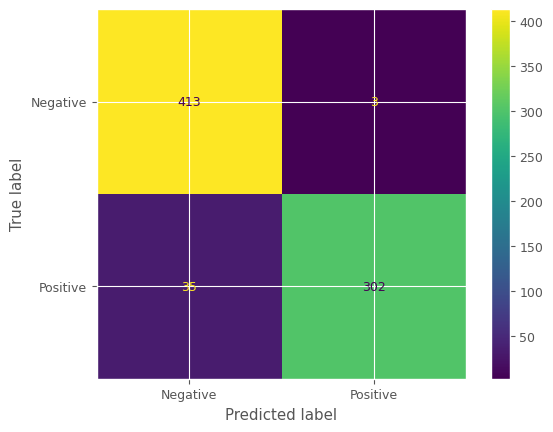
\includegraphics[width=\textwidth]{img/gnb/confusion_matrix_corr.png}
        \caption{Gaussian Naive Bayes allenato su dataset\_corr}
        \label{fig:matrice_di_confusione_per_GNB_corr}
    \end{subfigure}
    \hfill
    \begin{subfigure}{.45\textwidth}
        \centering
        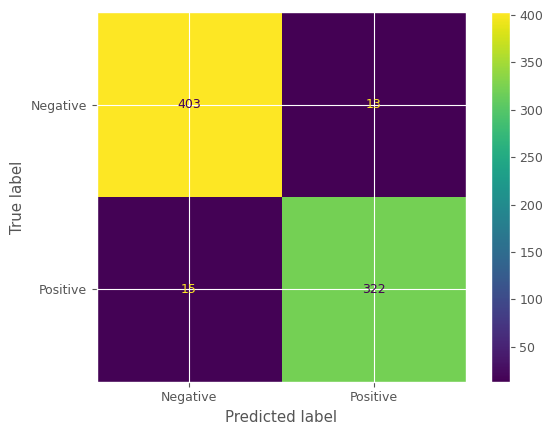
\includegraphics[width=\textwidth]{img/gnb/confusion_matrix_pca.png}
        \caption{Gaussian Naive Bayes allenato su dataset\_pca}
        \label{fig:matrice_di_confusione_per_GNB_pca}
    \end{subfigure}
    \caption{Matrici di confusione per Gaussian Naive Bayes}
    \label{fig:matrice_di_confusione_per_GNB}
\end{figure}

Le matrici di confusione evidenziano come i modelli generalizzano molto bene, più
precisamente il modello allenato su dataset\_corr ha un'accuracy del $95\%$, al 
contrario, quello allenato su dataset\_pca che raggiunge un'accuracy del $96\%$. 
Questo denota che ridurre le dimensioni del dataset utilizzando pca non porta a 
significativi miglioramenti sulle predizioni. Questo mancato miglioramento può 
essere dovuto al fatto che si è già trovata una buona ipotesi vicina alla 
funzione generatrice del dataset.

Dalle matrici di confusione oltre all'accuracy si possono calcolare le metriche
di precision, recall e F1-score, i loro valori sono visionabili nella tabella
\ref{tab:risultatiBayes}.

\begin{table}[!ht]
    \centering
    \begin{tabular}{@{}ccc@{}}
        \toprule
        \rowcolor[HTML]{EFEFEF} 
        \textbf{Metrica} & \textbf{Valore sul training set di dataset\_corr} & \textbf{Valore sul training set di dataset\_pca} \\ \midrule
        Accuracy  & 95\% & 96\% \\
        Precision & 90\% & 96\% \\
        Recall    & 99\% & 96\% \\
        F1-score  & 94\% & 96\% \\ \bottomrule
        \end{tabular}
    \caption{Metriche Gaussian Naive Bayes}
    \label{tab:risultatiBayes}
\end{table}

Dalle metriche di valutazione si può notare come su dataset\_corr si ha una 
precision minore rispetto alla recall, quindi significa che si tende ad associare 
la presenza di un tumore anche quando non è presente. Al contrario su dataset\_pca 
aumenta la precision diminuendo la recall, questo significa che sarà più 
affidabile su un riscontro positivo rispetto ad un riscontro negativo. In aggiunta, 
si può notare come F1-score è migliore nel modello allenato su dataset\_pca, 
questo potrebbe suggerire che, utilizzando pca, migliora la qualità delle 
predizioni. Il problema è che la metrica in questione calcola la media armonica 
tra precision e recall, ma nel dominio applicativo che si sta considerando, la 
recall assume maggior importanza dal momento che l'obiettivo è eliminare il falsi 
negativi e ammettere dei falsi positivi, perciò si dovrà massimizzare la recall.

Oltre alle metriche di valutazione sono stati prodotti i grafici delle curve ROC
di entrami i modelli, mostrati in figura \ref{fig:curve_roc}

\begin{figure}[!ht]
    \centering
    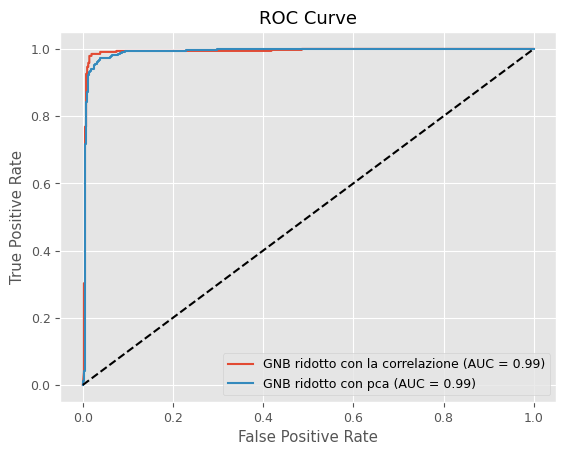
\includegraphics[width=.7\textwidth]{img/gnb/roc_curve.png}
    \caption{curve ROC}
    \label{fig:curve_roc}
\end{figure}

Le curve ROC permettono di confrontare i due modelli sfruttando la metrica AUC
che coincide con la misura dell'area sottesa alla curva del modello.
Come si può notare i due modelli hanno delle differenze non molto significative,
infatti entrambi hanno un'area AUC uguale, questo lascia intendere che siano
identici i due modelli. In realtà, AUC non considera la diversa importanza delle
classi, infatti, come anticipato precedentemente, nel dominio in questione un errore
di falso positivo ha un peso minore rispetto ad un faso negativo e questo criterio
di valutazione non viene considerato dalla metrica.

Bisogna specificare che questi studi sono stati realizzati su modelli che sono stati
allenati su un dataset di medie dimensioni ($\leq 10000$ esempi), perciò è stato
pensato di effettuare una valutazione dei modelli utilizzando la $10$-fold
stratified cross validation per poi ottenere gli intervalli di confidenza delle
metriche di valutazione i quali sono stati riportati in figura \ref{fig:intervalli_confidenza}.

\begin{figure}[!ht]
    \centering
    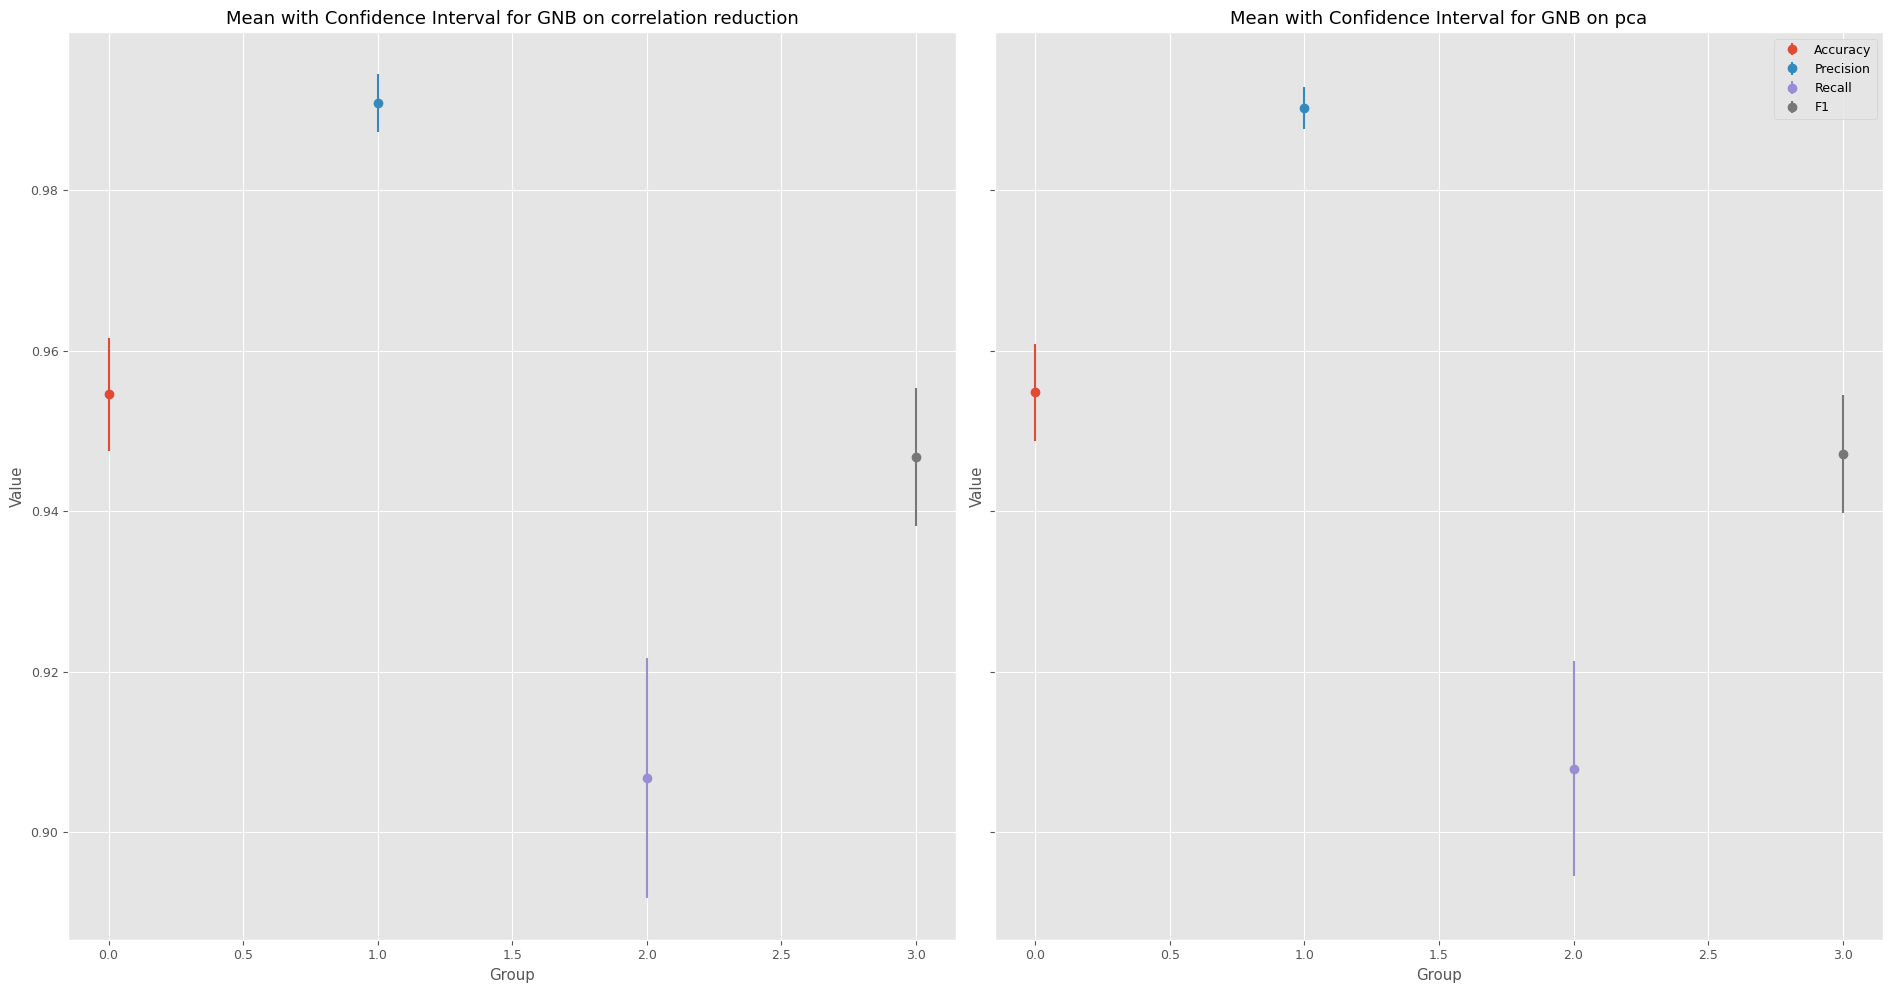
\includegraphics[width=\textwidth]{img/gnb/intervalli_confidenza.png}
    \caption{Intervalli di confidenza}
    \label{fig:intervalli_confidenza}
\end{figure}

Dagli intervalli di confidenza non ci sono significative differenze tra i due modelli,
quindi i ragionamenti svolti precedentemente sono confermati.